\documentclass{article}

\usepackage{titlesec}

\usepackage{amsmath}
\usepackage{amssymb}

\usepackage{booktabs}
\usepackage{float}
\usepackage{colortbl}
\usepackage{xcolor}

\usepackage{a4wide}
\usepackage{setspace}
\usepackage{geometry}
\usepackage{parskip}

\usepackage{multirow}
\usepackage{adjustbox}
\usepackage{graphicx}

\usepackage{hyperref}
\hypersetup{
    colorlinks=true,
    linkcolor=black,
    urlcolor=blue
}

\DeclareRobustCommand{\bbone}{\text{\usefont{U}{bbold}{m}{n}1}}

\titleformat*{\subsection}{\normalfont}

\author{Yu Xia \\ ID: yx5262}
\title{Yu Xia's Answer for Problem Set 5}
\date{Fall 2022}

\begin{document}
\maketitle

\nocite{*}

\section*{1}

\subsection*{(a)}

If $F_{0}\leqslant45$, investor enters the forward contract at $t=0$. The market value of investor's portfolio is 0. At $t=1$, he/she pays $F_{0}$ and sells ethanol on the spot.

Then in state 1, investor's payoff would be:

$65-F_{0}>0$

In state 2:

$45-F_{0}\geqslant0$

which is an arbitrage portfolio, a contradiction.

If $F_{0}\geqslant65$, investor enters the forward contract at $t=0$. The market value of investor's portfolio is 0. At $t=1$, he/she buys ethanol on the spot and sells at $F_{0}$ according to forward contract.

Then in state 1, investor's payoff would be:

$F_{0}-65\geqslant0$

In state 2:

$F_{0}-45>0$

which is an arbitrage portfolio, a contradiction.

In conclusion, $\boxed{F_{0}\in\left(45,65\right)}$

If there exist a risk neutral probability measure $\pi=\left\{\pi_{1}, \pi_{2}\right\}$ such that

$0=\dfrac{1}{1+r}\left(\pi_{1}\left(65-F_{0}\right)+\pi_{2}\left(45-F_{0}\right)\right)$

$1=\dfrac{1}{1+r}\left(\pi_{1}\left(1+r\right)+\pi_{2}\left(1+r\right)\right)\iff\pi_{1}+\pi_{2}=1$

$\implies0=\dfrac{1}{1+r}\left(\pi_{1}\left(65-F_{0}\right)+\left(1-\pi_{1}\right)\left(45-F_{0}\right)\right)$

$\pi_{1}\left(65-F_{0}\right)+\left(1-\pi_{1}\right)\left(45-F_{0}\right)=0$

$\pi_{1}\left(65-F_{0}\right)+\left(45-F_{0}\right)-\pi_{1}\left(45-F_{0}\right)=0$

$\pi_{1}\left[\left(65-F_{0}\right)-\left(45-F_{0}\right)\right]=F_{0}-45$

$\pi_{1}\left(65-F_{0}-45+F_{0}\right)=F_{0}-45$

$\pi_{1}=\boxed{\dfrac{F_{0}-45}{20}}$

$\pi_{2}=1-\pi_{1}=1-\dfrac{F_{0}-45}{20}=\dfrac{20}{20}-\dfrac{F_{0}-45}{20}=\dfrac{20-\left(F_{0}-45\right)}{20}=\dfrac{20-F_{0}+45}{20}=\boxed{\dfrac{65-F_{0}}{20}}$

\subsection*{(b)}

If $F_{0}\leqslant45$, investor enters the forward contract at $t=0$. The market value of investor's portfolio is 0. At $t=1$, he/she pays $F_{0}$ and sells ethanol on the spot.

Then in state 1, investor's pay off would be:

$65-F_{0}>0$

In state 2:

$45-F_{0}\geqslant0$

No matter which state investor is in, he/she makes money out of nothing. 

Similarly, if $F_{0}\geqslant65$, investor enters the forward contract at $t=0$. The market value of investor's portfolio is 0. At $t=1$, he/she buys ethanol on the spot and sells at $F_{0}$ according to forward contract.

Then in state 1, investor's payoff would be:

$F_{0}-65\geqslant0$

In state 2:

$F_{0}-45>0$

No matter which state investor is in, he/she makes money out of nothing. 

\subsection*{(c)}

The payoff matrix is:

$R=\begin{pmatrix}
    \rho_{1} & 1+r \\
    \rho_{2} & 1+r \\
    \rho_{3} & 1+r
\end{pmatrix}=\begin{pmatrix}
    65-F_{0} & 1+r \\
    45-F_{0} & 1+r \\
    55-F_{0} & 1+r
\end{pmatrix}$

Let the set of risk neutral probability measure $\pi=\left\{\pi_{1}, \pi_{2}, \pi_{3}\right\}$, \underline{where $\pi_{i}$ stands for the probability} \underline{of state $i$.}

$0=\pi_{1}\rho_{1}+\pi_{2}\rho_{2}+\pi_{3}\rho_{3}$

Substitude $1-\pi_{1}-\pi_{2}$ for $\pi_{3}$, we have:

$0=\pi_{1}\rho_{1}+\pi_{2}\rho_{2}+\left(1-\pi_{1}-\pi_{2}\right)\rho_{3}$

$0=\pi_{1}\rho_{1}+\pi_{2}\rho_{2}+\rho_{3}-\pi_{1}\rho_{3}-\pi_{2}\rho_{3}$

$0=\pi_{1}\left(\rho_{1}-\rho_{3}\right)+\pi_{2}\left(\rho_{2}-\rho_{3}\right)+\rho_{3}$

$-\pi_{2}\left(\rho_{2}-\rho_{3}\right)-\rho_{3}=\pi_{1}\left(\rho_{1}-\rho_{3}\right)$

$\pi_{1}\left(\rho_{1}-\rho_{3}\right)=-\pi_{2}\left(\rho_{2}-\rho_{3}\right)-\rho_{3}$

$\pi_{1}=\dfrac{-\pi_{2}\left(\rho_{2}-\rho_{3}\right)-\rho_{3}}{\rho_{1}-\rho_{3}}$

$\pi_{1}=\dfrac{\pi_{2}\left(\rho_{3}-\rho_{2}\right)-\rho_{3}}{\rho_{1}-\rho_{3}}$

$\pi_{3}=1-\pi_{1}-\pi_{2}=1-\dfrac{-\rho_{3}+\pi_{2}\left(\rho_{3}-\rho_{2}\right)}{\rho_{1}-\rho_{3}}-\pi_{2}$

$\pi_{3}=\dfrac{\rho_{1}-\rho_{3}}{\rho_{1}-\rho_{3}}+\dfrac{\rho_{3}-\pi_{2}\left(\rho_{3}-\rho_{2}\right)}{\rho_{1}-\rho_{3}}-\dfrac{\pi_{2}\left(\rho_{1}-\rho_{3}\right)}{\rho_{1}-\rho_{3}}$

$\pi_{3}=\dfrac{\rho_{1}-\rho_{3}+\rho_{3}-\left(\pi_{2}\rho_{3}-\pi_{2}\rho_{2}\right)-\left(\pi_{2}\rho_{1}-\pi_{2}\rho_{3}\right)}{\rho_{1}-\rho_{3}}$

$\pi_{3}=\dfrac{\rho_{1}-\pi_{2}\rho_{3}+\pi_{2}\rho_{2}-\pi_{2}\rho_{1}+\pi_{2}\rho_{3}}{\rho_{1}-\rho_{3}}$

$\pi_{3}=\dfrac{\rho_{1}+\pi_{2}\rho_{2}-\pi_{2}\rho_{1}}{\rho_{1}-\rho_{3}}$

$\pi_{3}=\dfrac{\rho_{1}+\pi_{2}\left(\rho_{2}-\rho_{1}\right)}{\rho_{1}-\rho_{3}}$

$\pi_{3}=\dfrac{\rho_{1}-\pi_{2}\left(\rho_{1}-\rho_{2}\right)}{\rho_{1}-\rho_{3}}$

$\because0<\pi_{1}=\dfrac{-\rho_{3}+\pi_{2}\left(\rho_{3}-\rho_{2}\right)}{\rho_{1}-\rho_{3}}<1$ and $\rho_{1}>\rho_{3}>\rho_{2}$

$\therefore0<-\rho_{3}+\pi_{2}\left(\rho_{3}-\rho_{2}\right)<\rho_{1}-\rho_{3}$

$\rho_{3}<\pi_{2}\left(\rho_{3}-\rho_{2}\right)<\rho_{1}-\rho_{3}+\rho_{3}=\rho_{1}$

$\dfrac{\rho_{3}}{\rho_{3}-\rho_{2}}<\pi_{2}<\dfrac{\rho_{1}}{\rho_{3}-\rho_{2}}$

$\because0<\pi_{3}=\dfrac{\rho_{1}-\pi_{2}\left(\rho_{1}-\rho_{2}\right)}{\rho_{1}-\rho_{3}}<1$

$\therefore0<\rho_{1}-\pi_{2}\left(\rho_{1}-\rho_{2}\right)<\rho_{1}-\rho_{3}$

$\rho_{3}-\rho_{1}<-\rho_{1}+\pi_{2}\left(\rho_{1}-\rho_{2}\right)<0$

$\rho_{3}-\rho_{1}+\rho_{1}=\rho_{3}<\pi_{2}\left(\rho_{1}-\rho_{2}\right)<\rho_{1}$

$\dfrac{\rho_{3}}{\rho_{1}-\rho_{2}}<\pi_{2}<\dfrac{\rho_{1}}{\rho_{1}-\rho_{2}}$

$\because\rho_{1}>\rho_{3}>\rho_{2}$

$\therefore\rho_{1}-\rho_{2}>\rho_{3}-\rho_{2}$

$\dfrac{\rho_{1}}{\rho_{1}-\rho_{2}}<\dfrac{\rho_{1}}{\rho_{3}-\rho_{2}}$

$\dfrac{\rho_{3}}{\rho_{3}-\rho_{2}}>\dfrac{\rho_{3}}{\rho_{1}-\rho_{2}}$

Thus,

$\dfrac{\rho_{3}}{\rho_{3}-\rho_{2}}<\pi_{2}<\dfrac{\rho_{1}}{\rho_{1}-\rho_{2}}$

$\because \pi_{2}\in\left(0,1\right)$

$\therefore\dfrac{\rho_{3}}{\rho_{3}-\rho_{2}}<1$

$\rho_{3}<\rho_{3}-\rho_{2}$

$\rho_{2}<0$

On the other hand,

$\dfrac{\rho_{1}}{\rho_{1}-\rho_{2}}>0$

$\rho_{1}>0$

Plug in we have:

$\rho_{3}-\rho_{2}=10$

$\rho_{1}-\rho_{3}=10$

$\rho_{1}-\rho_{2}=20$

$\pi_{1}=\dfrac{10\pi_{2}-\left(55-F_{0}\right)}{10}=\dfrac{10\pi_{2}-55+F_{0}}{10}$

$\pi_{3}=\dfrac{65-F_{0}-20\pi_{2}}{10}$

$\dfrac{55-F_{0}}{10}<\pi_{2}<\dfrac{65-F_{0}}{20}$

$\rho_{2}<0 \implies F_{0}>45$

$\rho_{1}>0 \implies F_{0}<65$

\fbox{%
\parbox[c]{.5\textwidth}{
$\pi_{1}=\dfrac{10\pi_{2}-55+F_{0}}{10}$

$\pi_{3}=\dfrac{65-F_{0}-20\pi_{2}}{10}$

$\dfrac{55-F_{0}}{10}<\pi_{2}<\dfrac{65-F_{0}}{20}$

$45<F_{0}<65$
}}

\section*{2}

\subsection*{(a)}

The arbitrage free forward price per pound, denote as $f_{0}$, is given by the equation:

$0=\dfrac{1}{\left(1+0.4\%\right)^{2}}\left(\left(0.5\right)^{2}\left(1.28-f_{0}\right)+2\left(0.5\right)^{2}\left(1.24-f_{0}\right)+\left(0.5\right)^{2}\left(1.20-f_{0}\right)\right)$

$0=0.25\left(1.28-f_{0}\right)+0.5\left(1.24-f_{0}\right)+0.25\left(1.20-f_{0}\right)$

$0=\left(1.28-f_{0}\right)+2\left(1.24-f_{0}\right)+\left(1.20-f_{0}\right)$

$\left(1+2+1\right)f_{0}=1.28+2\times1.24+1.20$

$4f_{0}=1.28+2.48+1.20=4.96$

$f_{0}=1.24$

$\therefore F_{0}=50,000f_{0}=50,000\times1.24=\boxed{62,000}$

\subsection*{(b)}

By the no-arbitrage pricing formula, we have:

\begin{multline*}
    0=\dfrac{1}{1+r}\left(\pi\dfrac{\Phi_{1u}-\Phi_{0}}{1000}+\left(1-\pi\right)\dfrac{\Phi_{1d}-\Phi_{0}}{1000}\right)\\
    +\dfrac{\pi}{\left(1+r\right)^{2}}\left(\pi\left(1.28-\dfrac{\Phi_{1u}}{1000}\right)+\left(1-\pi\right)\left(1.24-\dfrac{\Phi_{1u}}{1000}\right)\right)\\
    +\dfrac{1-\pi}{\left(1+r\right)^{2}}\left(\pi\left(1.24-\dfrac{\Phi_{1d}}{1000}\right)+\left(1-\pi\right)\left(1.20-\dfrac{\Phi_{1d}}{1000}\right)\right)
\end{multline*}

and

$0=\dfrac{1}{1+r}\left(\pi\left(1.28-\dfrac{\Phi_{1u}}{1000}\right)+\left(1-\pi\right)\left(1.24-\dfrac{\Phi_{1u}}{1000}\right)\right)$

$\implies0=\pi\left(1280-\Phi_{1u}\right)+\left(1-\pi\right)\left(1240-\Phi_{1u}\right)$

$\implies0=1280\pi-\Phi_{1u}\pi+1240\left(1-\pi\right)-\Phi_{1u}\left(1-\pi\right)$

$\implies0=1280\pi+1240-1240\pi-\Phi_{1u}$

$\implies\Phi_{1u}=1280\pi+1240\left(1-\pi\right)=\boxed{40\pi+1240}$

also

$0=\dfrac{1}{1+r}\left(\pi\left(1.24-\dfrac{\Phi_{1d}}{1000}\right)+\left(1-\pi\right)\left(1.20-\dfrac{\Phi_{1d}}{1000}\right)\right)$

$\implies0=\pi\left(1240-\Phi_{1d}\right)+\left(1-\pi\right)\left(1200-\Phi_{1d}\right)$

$\implies\Phi_{1d}=1240\pi+1200\left(1-\pi\right)=\boxed{1200+40\pi}$

$\therefore1.28-\dfrac{\Phi_{1u}}{1000}=1.28-\left(0.04\pi+1.24\right)=1.28-0.04\pi-1.24=0.04-0.04\pi$

$1280-\Phi_{1u}=40-40\pi$

$1.24-\dfrac{\Phi_{1u}}{1000}=-0.04\pi$

$1240-\Phi_{1u}=-40\pi$

$1.24-\dfrac{\Phi_{1d}}{1000}=1.24-\left(1.20+0.04\pi\right)=1.24-1.20-0.04\pi=0.04-0.04\pi$

$1240-\Phi_{1d}=40-40\pi$

$1.20-\dfrac{\Phi_{1d}}{1000}=-0.04\pi$

$1200-\Phi_{1d}=-40\pi$

Thus

\begin{multline*}
    0=\dfrac{1}{1+r}\left(\pi\left(0.04\pi+1.24-\dfrac{\Phi_{0}}{1000}\right)+\left(1-\pi\right)\left(1.20+0.04\pi-\dfrac{\Phi_{0}}{1000}\right)\right)\\
    +\dfrac{\pi}{\left(1+r\right)^{2}}\left(\pi\left(0.04-0.04\pi\right)+\left(1-\pi\right)\left(-0.04\pi\right)\right)\\
    +\dfrac{1-\pi}{\left(1+r\right)^{2}}\left(\pi\left(0.04-0.04\pi\right)+\left(1-\pi\right)\left(-0.04\pi\right)\right)
\end{multline*}
$\implies$
\begin{multline*}
    0=\dfrac{1}{1+r}\left(\pi\left(0.04\pi+1.24-\dfrac{\Phi_{0}}{1000}\right)+\left(1-\pi\right)\left(1.20+0.04\pi-\dfrac{\Phi_{0}}{1000}\right)\right)\\
    +\dfrac{1}{\left(1+r\right)^{2}}\left(\pi\left(0.04-0.04\pi\right)+\left(1-\pi\right)\left(-0.04\pi\right)\right)
\end{multline*}
$\implies$
\begin{multline*}
    0=\left(\pi\left(0.04\pi+1.24-\dfrac{\Phi_{0}}{1000}\right)+\left(1-\pi\right)\left(1.20+0.04\pi-\dfrac{\Phi_{0}}{1000}\right)\right)\\
    +\dfrac{1}{1+r}\left(\pi\left(0.04-0.04\pi\right)+\left(1-\pi\right)\left(-0.04\pi\right)\right)
\end{multline*}
$\implies$
\begin{multline*}
    0=\pi\left(0.04\pi+1.24-\dfrac{\Phi_{0}}{1000}\right)+\left(1-\pi\right)\left(1.20+0.04\pi-\dfrac{\Phi_{0}}{1000}\right)\\
    -\dfrac{1}{1+r}\left(\pi\left(0.04\pi-0.04\right)+\left(1-\pi\right)\left(0.04\pi\right)\right)
\end{multline*}
$\implies$
\begin{multline*}
    \dfrac{1}{1+r}\left(\pi\left(0.04\pi-0.04\right)+\left(1-\pi\right)\left(0.04\pi\right)\right)\\
    =\pi\left(0.04\pi+1.24-\dfrac{\Phi_{0}}{1000}\right)+\left(1-\pi\right)\left(1.20+0.04\pi-\dfrac{\Phi_{0}}{1000}\right)
\end{multline*}
$\implies$
\begin{multline*}
    \dfrac{1}{1+r}\left(\left(0.04\pi^{2}-0.04\pi\right)+\left(0.04\pi-0.04\pi^{2}\right)\right)\\
    =\pi\left(1.24+0.04\pi-\dfrac{\Phi_{0}}{1000}\right)+\left(1-\pi\right)\left(1.20+0.04\pi-\dfrac{\Phi_{0}}{1000}\right)
\end{multline*}
$\implies$
\begin{multline*}
    \dfrac{1}{1+r}\left(0.04\pi^{2}-0.04\pi+0.04\pi-0.04\pi^{2}\right)\\
    =1.24\pi+\pi\left(0.04\pi-\dfrac{\Phi_{0}}{1000}\right)+1.20\left(1-\pi\right)+\left(1-\pi\right)\left(0.04\pi-\dfrac{\Phi_{0}}{1000}\right)
\end{multline*}

$\implies0=1.24\pi+1.20-1.20\pi+0.04\pi-\dfrac{\Phi_{0}}{1000}$

$\implies\Phi_{0}=40\pi+1200+40\pi$

$\implies\boxed{\Phi_{0}=80\pi+1200}$

$\Phi_{1u}-\Phi_{0}=40\pi+1240-\left(80\pi+1200\right)=40-40\pi$

$\Phi_{1d}-\Phi_{0}=1200+40\pi-\left(80\pi+1200\right)=-40\pi$

\begin{figure}[H]
    \begin{center}
        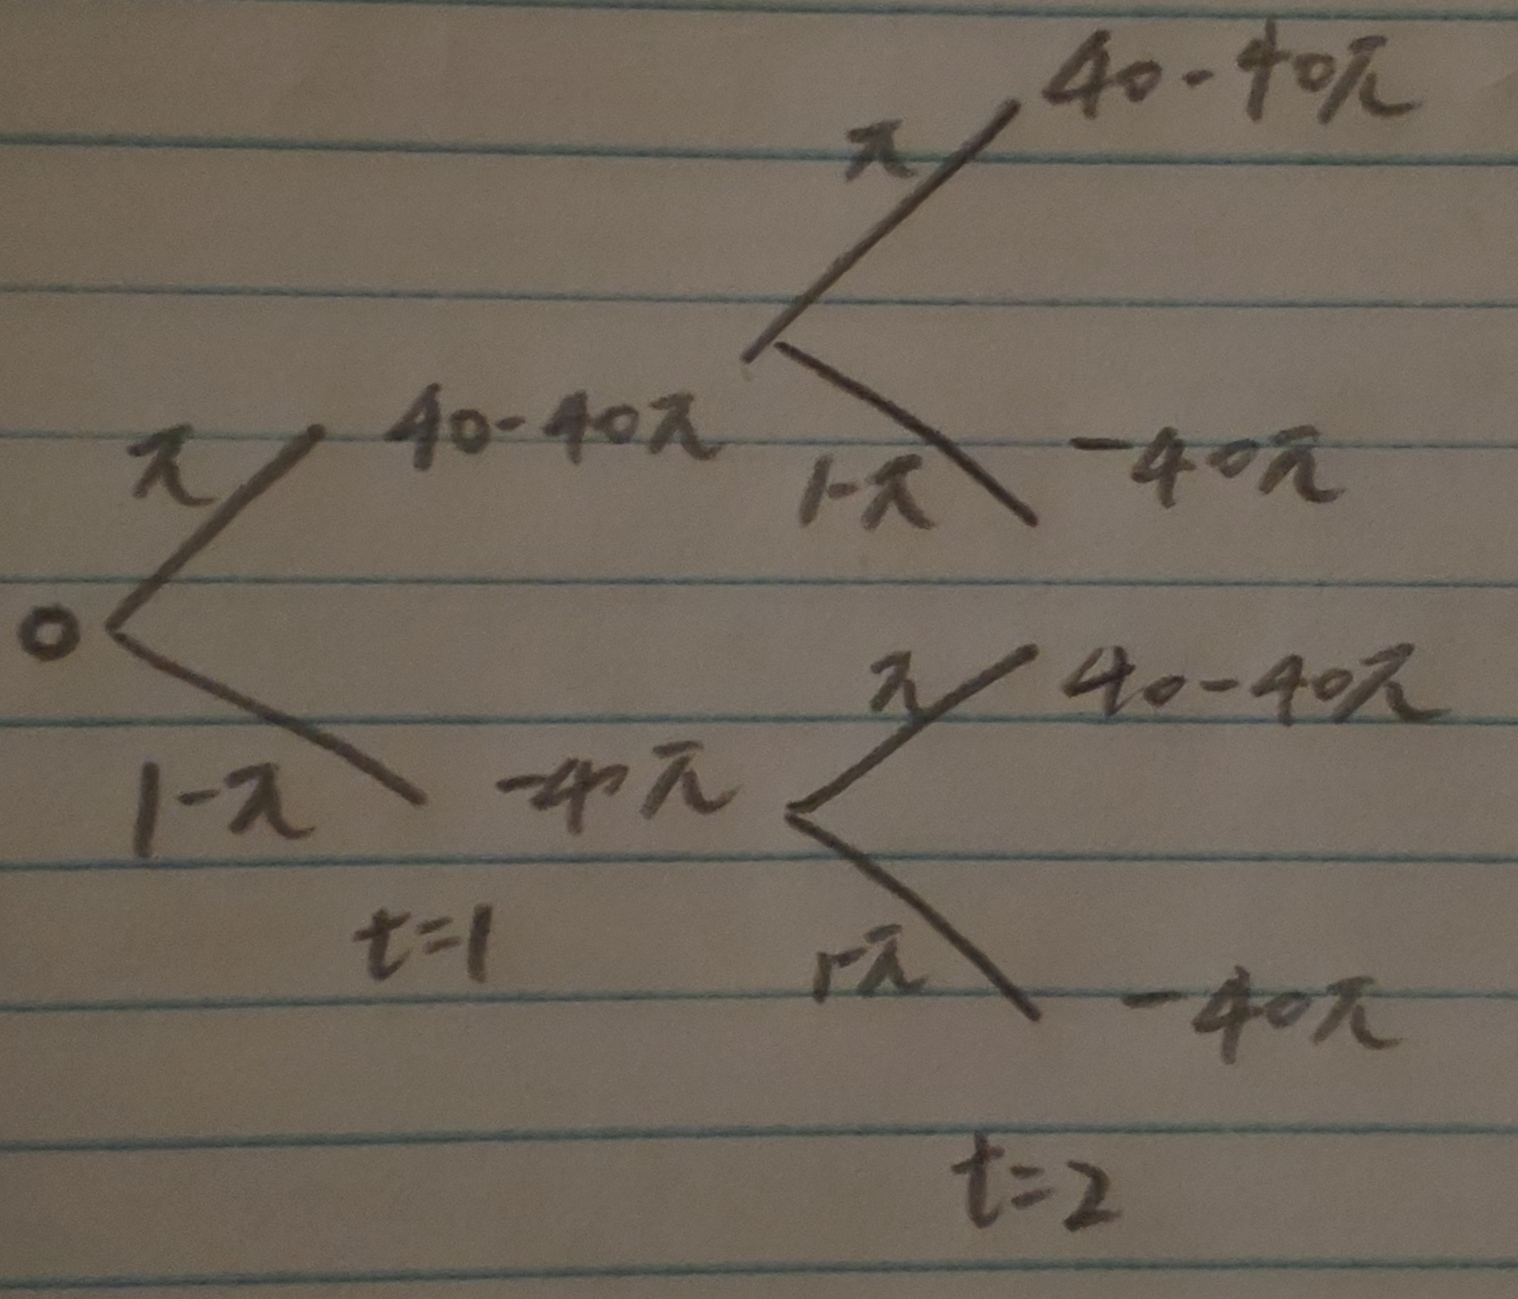
\includegraphics[width=1\textwidth]{figures/1665780213537.jpg}
    \end{center}
    \caption{Time-decision tree of (b)}
    \label{fig:graph}
\end{figure}

\subsection*{(c)}

Similarly,

\begin{multline*}
    0=\dfrac{1}{1+r}\left(\pi\left(1.26-X\right)+\left(1-\pi\right)\left(1.22-X\right)\right)\\
    +\dfrac{\pi}{\left(1+r\right)^{2}}\left(\pi\left(1.28-X\right)+\left(1-\pi\right)\left(1.24-X\right)\right)\\
    +\dfrac{1-\pi}{\left(1+r\right)^{2}}\left(\pi\left(1.24-X\right)+\left(1-\pi\right)\left(1.20-X\right)\right)
\end{multline*}

\begin{multline*}
    0=\dfrac{1}{1+r}\left(\left(1.26\pi-X\pi\right)+\left(1.22\left(1-\pi\right)-X\left(1-\pi\right)\right)\right)\\
    +\dfrac{\pi}{\left(1+r\right)^{2}}\left(\left(1.28\pi-X\pi\right)+\left(1.24\left(1-\pi\right)-X\left(1-\pi\right)\right)\right)\\
    +\dfrac{1-\pi}{\left(1+r\right)^{2}}\left(\left(1.24\pi-X\pi\right)+\left(1.20\left(1-\pi\right)-X\left(1-\pi\right)\right)\right)
\end{multline*}

\begin{multline*}
    0=\dfrac{1}{1+r}\left(\left(1.26\pi-X\pi\right)+\left(\left(1.22-1.22\pi\right)-\left(X-X\pi\right)\right)\right)\\
    +\dfrac{\pi}{\left(1+r\right)^{2}}\left(\left(1.28\pi-X\pi\right)+\left(\left(1.24-1.24\pi\right)-\left(X-X\pi\right)\right)\right)\\
    +\dfrac{1-\pi}{\left(1+r\right)^{2}}\left(\left(1.24\pi-X\pi\right)+\left(\left(1.20-1.20\pi\right)-\left(X-X\pi\right)\right)\right)
\end{multline*}

\begin{multline*}
    0=\dfrac{1}{1+r}\left(1.26\pi-X\pi+1.22-1.22\pi-X+X\pi\right)\\
    +\dfrac{\pi}{\left(1+r\right)^{2}}\left(1.28\pi-X\pi+1.24-1.24\pi-X+X\pi\right)\\
    +\dfrac{1-\pi}{\left(1+r\right)^{2}}\left(1.24\pi-X\pi+1.20-1.20\pi-X+X\pi\right)
\end{multline*}

\begin{multline*}
    0=\dfrac{1}{1+r}\left(1.26\pi+1.22-1.22\pi-X\right)\\
    +\dfrac{\pi}{\left(1+r\right)^{2}}\left(1.28\pi+1.24-1.24\pi-X\right)\\
    +\dfrac{1-\pi}{\left(1+r\right)^{2}}\left(1.24\pi+1.20-1.20\pi-X\right)
\end{multline*}

\begin{equation*}
    0=\dfrac{1}{1+r}\left(0.04\pi+1.22-X\right)+\dfrac{\pi}{\left(1+r\right)^{2}}\left(0.04\pi+1.24-X\right)+\dfrac{1-\pi}{\left(1+r\right)^{2}}\left(0.04\pi+1.20-X\right)
\end{equation*}

\begin{equation*}
    0=\left(0.04\pi+1.22-X\right)+\dfrac{\pi}{1+r}\left(0.04\pi+1.24-X\right)+\dfrac{1-\pi}{1+r}\left(0.04\pi+1.20-X\right)
\end{equation*}

\begin{multline*}
    0=\left(0.04\pi+1.22-X\right)+\dfrac{1}{1+r}\left(0.04\pi^{2}+1.24\pi-X\pi\right)\\
    +\dfrac{1}{1+r}\left(0.04\pi\left(1-\pi\right)+1.20\left(1-\pi\right)-X\left(1-\pi\right)\right)
\end{multline*}

\begin{multline*}
    0=\left(1+r\right)\left(0.04\pi+1.22-X\right)+\left(0.04\pi^{2}+1.24\pi-X\pi\right)\\
    +\left(0.04\pi-0.04\pi^{2}+1.20-1.20\pi-\left(X-X\pi\right)\right)
\end{multline*}

\begin{multline*}
    0=\left(0.04\pi\left(1+r\right)+1.22\left(1+r\right)-X\left(1+r\right)\right)+\left(0.04\pi^{2}+1.24\pi-X\pi\right)\\
    +\left(0.04\pi-0.04\pi^{2}+1.20-1.20\pi-X+X\pi\right)
\end{multline*}

\begin{multline*}
    0=0.04\pi+0.04\pi r+1.22+1.22r-\left(X+Xr\right)+0.04\pi^{2}+1.24\pi-X\pi\\
    +0.04\pi-0.04\pi^{2}+1.20-1.20\pi-X+X\pi
\end{multline*}

\begin{equation*}
    0=0.04\pi+0.04\pi r+1.22+1.22r-X-Xr+1.24\pi+0.04\pi+1.20-1.20\pi-X
\end{equation*}

\begin{equation*}
    0=1.22+1.20+0.04\pi+1.24\pi+0.04\pi-1.20\pi+0.04\pi r+1.22r-Xr-X-X
\end{equation*}

\begin{equation*}
    X\left(2+r\right)=2.42+0.12\pi+0.04\pi r+1.22r
\end{equation*}

\begin{equation*}
    \boxed{X=\dfrac{2.42+0.12\pi+0.04\pi r+1.22r}{2+r}}
\end{equation*}

$25,000X=\dfrac{60,500+3,000\pi+1,000\pi r+30,500r}{2+r}$

\begin{flalign*}
    25,000\left(1.26-X\right) &=25,000\left(\dfrac{1.26\left(2+r\right)}{2+r}-\dfrac{2.42+0.12\pi+0.04\pi r+1.22r}{2+r}\right)&\\
    &=25,000\times\dfrac{2.52+1.26r-2.42-0.12\pi-0.04\pi r-1.22r}{2+r} &\\
    &=25,000\times\dfrac{0.1+0.04r-0.12\pi-0.04\pi r}{2+r} &\\
    &=\dfrac{2,500+1,000r-3,000\pi-1,000\pi r}{2+r}
\end{flalign*}

\begin{flalign*}
    25,000\left(1.22-X\right) &=25,000\left(\dfrac{1.22\left(2+r\right)}{2+r}-\dfrac{2.42+0.12\pi+0.04\pi r+1.22r}{2+r}\right)&\\
    &=25,000\times\dfrac{2.44+1.26r-2.42-0.12\pi-0.04\pi r-1.22r}{2+r} &\\
    &=25,000\times\dfrac{0.02+0.04r-0.12\pi-0.04\pi r}{2+r} &\\
    &=\dfrac{500+1,000r-3,000\pi-1,000\pi r}{2+r}
\end{flalign*}

\begin{flalign*}
    25,000\left(1.28-X\right) &=25,000\left(\dfrac{1.28\left(2+r\right)}{2+r}-\dfrac{2.42+0.12\pi+0.04\pi r+1.22r}{2+r}\right)&\\
    &=25,000\times\dfrac{2.56+1.26r-2.42-0.12\pi-0.04\pi r-1.22r}{2+r} &\\
    &=25,000\times\dfrac{0.14+0.04r-0.12\pi-0.04\pi r}{2+r} &\\
    &=\dfrac{3,500+1,000r-3,000\pi-1,000\pi r}{2+r}
\end{flalign*}

\begin{flalign*}
    25,000\left(1.24-X\right) &=25,000\left(\dfrac{1.24\left(2+r\right)}{2+r}-\dfrac{2.42+0.12\pi+0.04\pi r+1.22r}{2+r}\right)&\\
    &=25,000\times\dfrac{2.48+1.26r-2.42-0.12\pi-0.04\pi r-1.22r}{2+r} &\\
    &=25,000\times\dfrac{0.06+0.04r-0.12\pi-0.04\pi r}{2+r} &\\
    &=\dfrac{1,500+1,000r-3,000\pi-1,000\pi r}{2+r}
\end{flalign*}

\begin{flalign*}
    25,000\left(1.20-X\right) &=25,000\left(\dfrac{1.2\left(2+r\right)}{2+r}-\dfrac{2.42+0.12\pi+0.04\pi r+1.22r}{2+r}\right)&\\
    &=25,000\times\dfrac{2.4+1.26r-2.42-0.12\pi-0.04\pi r-1.22r}{2+r} &\\
    &=25,000\times\dfrac{-0.02+0.04r-0.12\pi-0.04\pi r}{2+r} &\\
    &=\dfrac{-500+1,000r-3,000\pi-1,000\pi r}{2+r}
\end{flalign*}

\begin{figure}[H]
    \begin{center}
        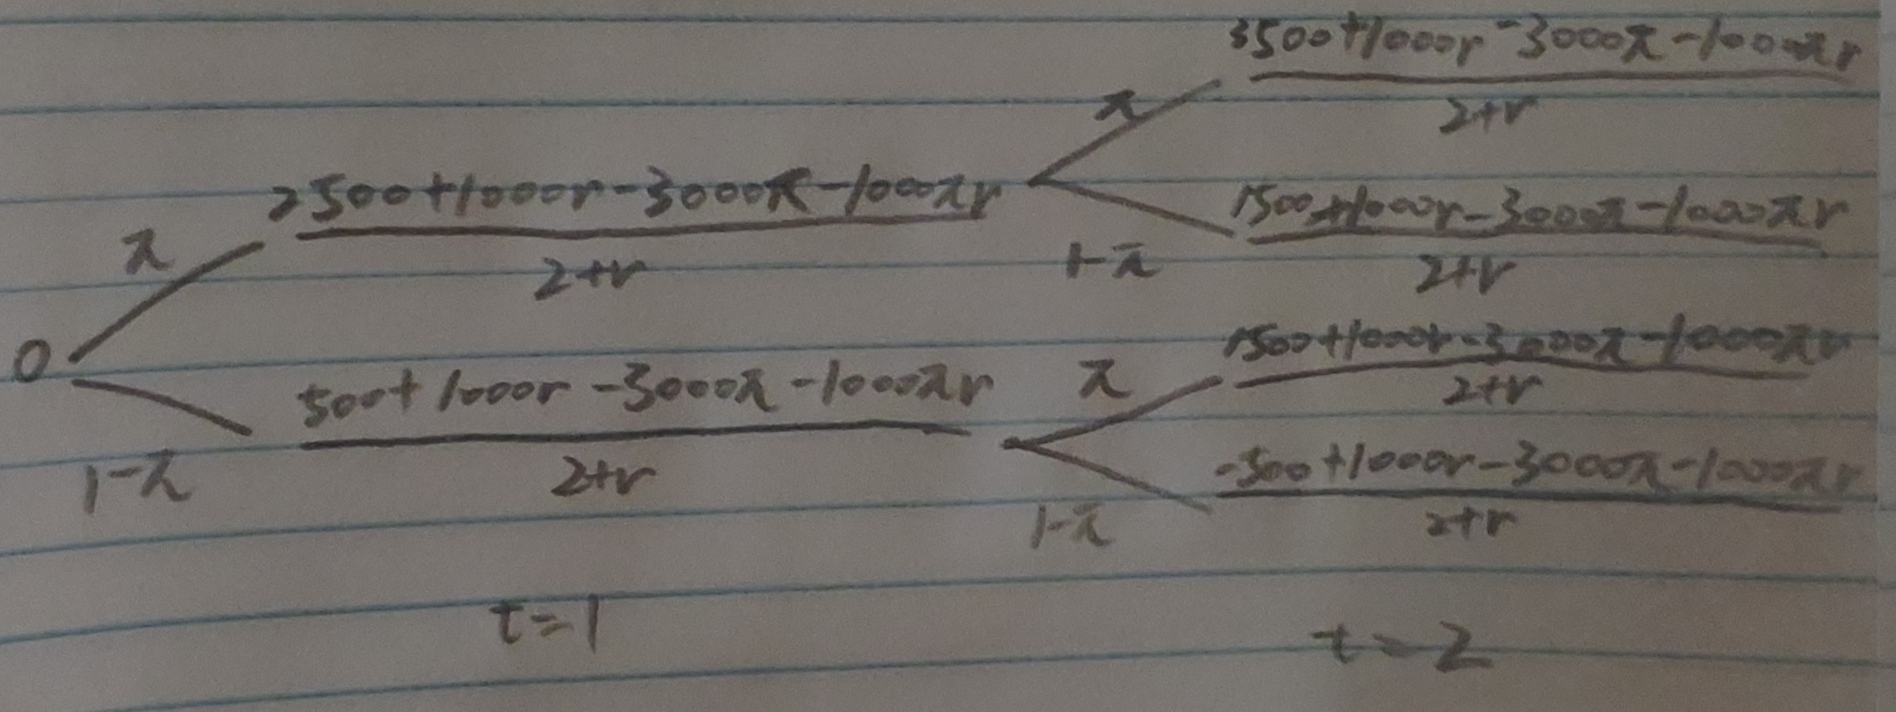
\includegraphics[width=1\textwidth]{figures/1665780213526.jpg}
    \end{center}
    \caption{Time-decision tree of (c)}
    \label{fig:graph}
\end{figure}

\section*{3}

\subsection*{(a)}

Let the risk-neutral probability measure $\pi=\left(\pi_{1},\pi_{2}\right)$.

We have

$\pi_{1}+\pi_{2}=1\implies\pi_{2}=1-\pi_{1}$

Look at the stock at first.

If this stock is arbitrage free, by the pricing formula (1.2) in the lecture note, we get:

$\boxed{q_{1}=\dfrac{\pi_{1}gq_{1}+\left(1-\pi_{1}\right)bq_{1}}{1+r}}$

$\implies\left(1+r\right)q_{1}=\pi_{1}gq_{1}+bq_{1}-\pi_{1}bq_{1}$

$\implies\left(1+r\right)q_{1}-bq_{1}=\pi_{1}\left(gq_{1}-bq_{1}\right)$

$\implies \pi_{1}=\dfrac{\left(1+r\right)q_{1}-bq_{1}}{gq_{1}-bq_{1}}$

\begin{flalign*}
    \pi_{2} &=1-\pi_{1} &\\
    &=\dfrac{gq_{1}-bq_{1}}{gq_{1}-bq_{1}}-\dfrac{\left(1+r\right)q_{1}-bq_{1}}{gq_{1}-bq_{1}} &\\
    &=\dfrac{gq_{1}-bq_{1}-\left(\left(1+r\right)q_{1}-bq_{1}\right)}{gq_{1}-bq_{1}} &\\
    &=\dfrac{gq_{1}-bq_{1}-\left(1+r\right)q_{1}+bq_{1}}{gq_{1}-bq_{1}} &\\
    &=\dfrac{gq_{1}-\left(1+r\right)q_{1}}{gq_{1}-bq_{1}}
\end{flalign*}

$\because \pi_{1}\geqslant0, \pi_{2}\geqslant0$

$\therefore \dfrac{\left(1+r\right)q_{1}-bq_{1}}{gq_{1}-bq_{1}}\geqslant0, \dfrac{gq_{1}-\left(1+r\right)q_{1}}{gq_{1}-bq_{1}}\geqslant0$

$\because g>b$

$\therefore gq_{1}-bq_{1}>0$

$\implies \left(1+r\right)q_{1}-bq_{1}\geqslant0, gq_{1}-\left(1+r\right)q_{1}\geqslant0$

$\implies \left(1+r\right)q_{1}\geqslant bq_{1}, gq_{1}\geqslant\left(1+r\right)q_{1}$

$\implies q_{1}\geqslant\dfrac{bq_{1}}{1+r}, q_{1}\leqslant\dfrac{gq_{1}}{1+r}$

$\implies \dfrac{bq_{1}}{1+r}\leqslant q_{1}\leqslant\dfrac{gq_{1}}{1+r}$

$\implies \dfrac{b}{1+r}\leqslant1\leqslant\dfrac{g}{1+r}$

$1-\dfrac{g}{1+r}\leqslant0$, and $1-\dfrac{b}{1+r}\geqslant0$

$\left(1+r\right)-g\leqslant0$, and $\left(1+r\right)-b\geqslant0$

$\therefore \boxed{\dfrac{\left(1+r\right)-g}{\left(1+r\right)-b}\leqslant0}$

In order to make sure that $\pi_{1}\leqslant1$ and $\pi_{2}\leqslant1$, $g>b\geqslant1+r$.

\subsection*{(b)}

If $K\geqslant\max\left\{r_{11}, r_{21}\right\}=gq_{1}$, the buyer always choose to put. 

If $K\leqslant\min\left\{r_{11}, r_{21}\right\}=bq_{1}$, the buyer always choose not to put. 

If $bq_{1}<K<gq_{1}$,

Let $\alpha_{p}$ be the shares of the stock, $\beta_{p}$ be the shares of the bond.

We have the system of equation:

$0=gq_{1}\alpha_{p}+Rq_{2}\beta_{p}$

$K-bq_{1}=bq_{1}\alpha_{p}+Rq_{2}\beta_{p}$

$\implies$

$bq_{1}-K=\left(g-b\right)q_{1}\alpha_{p}$

$\alpha_{p}=\dfrac{bq_{1}-K}{\left(g-b\right)q_{1}}$

$Rq_{2}\beta_{p}=-gq_{1}\alpha_{p}=-gq_{1}\cdot\dfrac{bq_{1}-K}{\left(g-b\right)q_{1}}=g\cdot\dfrac{K-bq_{1}}{g-b}=\dfrac{g\left(K-bq_{1}\right)}{g-b}$

$\beta_{p}=\dfrac{g\left(K-bq_{1}\right)}{Rq_{2}\left(g-b\right)}$

$\therefore q_{3}=q_{1}\alpha_{p}+q_{2}\beta_{p}=q_{1}\dfrac{bq_{1}-K}{\left(g-b\right)q_{1}}+q_{2}\dfrac{g\left(K-bq_{1}\right)}{Rq_{2}\left(g-b\right)}=\boxed{\dfrac{bq_{1}-K}{g-b}+\dfrac{g\left(K-bq_{1}\right)}{R\left(g-b\right)}}$

On the other hand,

$q_{1}=\dfrac{1}{R}\left(\pi_{1}gq_{1}+\pi_{2}bq_{1}\right)=\dfrac{1}{R}\left(\pi_{1}gq_{1}+\left(1-\pi_{1}\right)bq_{1}\right)=\dfrac{1}{R}\left(\pi_{1}gq_{1}+bq_{1}-\pi_{1}bq_{1}\right)=\dfrac{q_{1}}{R}\left(\pi_{1}\left(g-b\right)+b\right)$

$\implies R=\pi_{1}\left(g-b\right)+b\implies\pi_{1}\left(g-b\right)=R-b$

$\implies\boxed{\pi_{1}=\dfrac{R-b}{g-b}}$

$\implies\pi_{2}=1-\pi_{1}=1-\dfrac{R-b}{g-b}=\dfrac{g-b}{g-b}-\dfrac{R-b}{g-b}=\dfrac{g-b-\left(R-b\right)}{g-b}=\dfrac{g-b-R+b}{g-b}$

$\boxed{\pi_{2}=\dfrac{g-R}{g-b}}$

$\mathbb{E}^{\pi}\left[r_{3}\right]=\pi_{1}r_{13}+\pi_{2}r_{23}=0+\dfrac{g-R}{g-b}\cdot\left(K-bq_{1}\right)=\dfrac{g\left(K-bq_{1}\right)}{g-b}-\dfrac{R\left(K-bq_{1}\right)}{g-b} $

$R^{-1}\mathbb{E}^{\pi}\left[r_{3}\right]=\dfrac{g\left(K-bq_{1}\right)}{R\left(g-b\right)}-\dfrac{K-bq_{1}}{g-b}=\dfrac{g\left(K-bq_{1}\right)}{R\left(g-b\right)}+\dfrac{bq_{1}-K}{g-b}=q_{3}$

\end{document}